\section{Free Fibonacci chain at high energy}
\subsection{Dummy}
\begin{frame}{Interacting fermions on the Fibonacci chain}
{

\centering
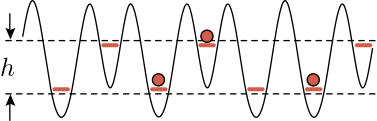
\includegraphics[width=0.4\textwidth]{img/3_Fibonacci/XXZ_QP_cold_atoms}
\[
	H = \sum_{i=1}^L \left[ J (c_i^\dagger c_{i+1} + \text{h.c}) + \Delta n_i n_{i+1} - h_i n_i \right]
\]
}

\begin{block}{Method: numerical \textbf{exact diagonalization}}
\begin{itemize}
	\item High energy + non-integrable: \textbf{no analytical methods}
	\item $L/2$ fermions on $L$ sites: $\# \text{states} \sim 2^L/\sqrt{L} \to$ \textbf{memory is limiting}

State-of-the art: $L=24$ {\footnotesize[Pietracaprina \emph{et al} 18]}

	\item Fibonacci: \textbf{few samples}: $L/2$ non-equivalent systems of size $L$.
\end{itemize}
\end{block}
\end{frame}

\begin{frame}{Free fermions properties}
\begin{itemize}
	\item Multifractal single particle wavefunctions {\footnotesize[Ostlund; Kalugin; Kohmoto; \dots]}
	\item Anomalous transport {\footnotesize[Mayou; Schreiber; Varma \& Žnidarič; \dots]}
\end{itemize}
\begin{columns}
\begin{column}{0.5\textwidth}
\centering
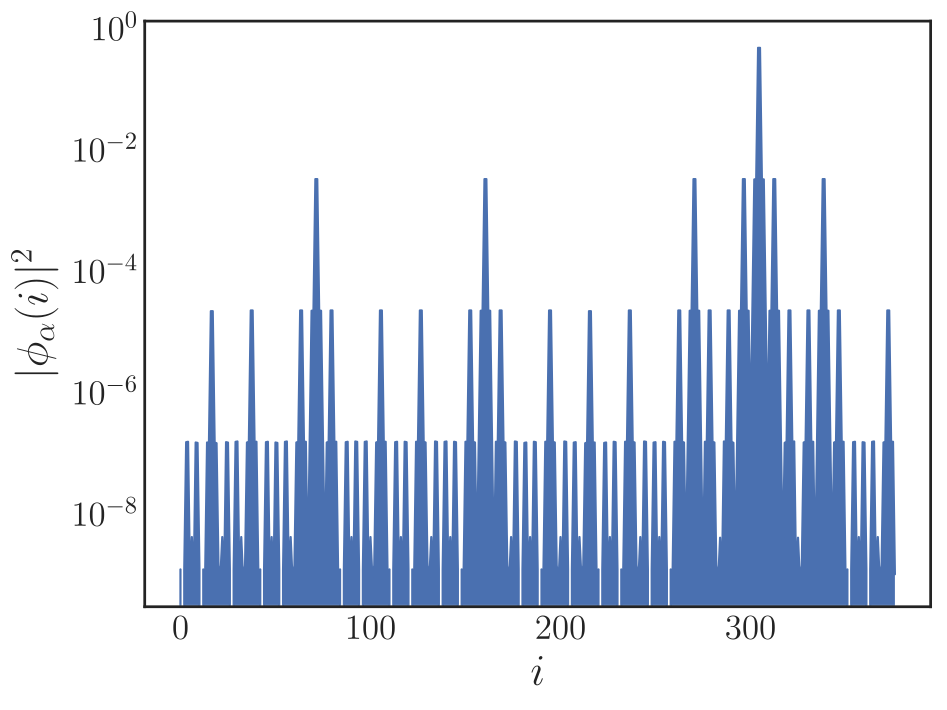
\includegraphics[width=0.8\textwidth]{img/3_Fibonacci/presence_prob}

{\footnotesize Single particle wavefunction at the Fermi level}
\end{column}
%%%%%%%%%%%%%%%%%%
\begin{column}{0.5\textwidth}
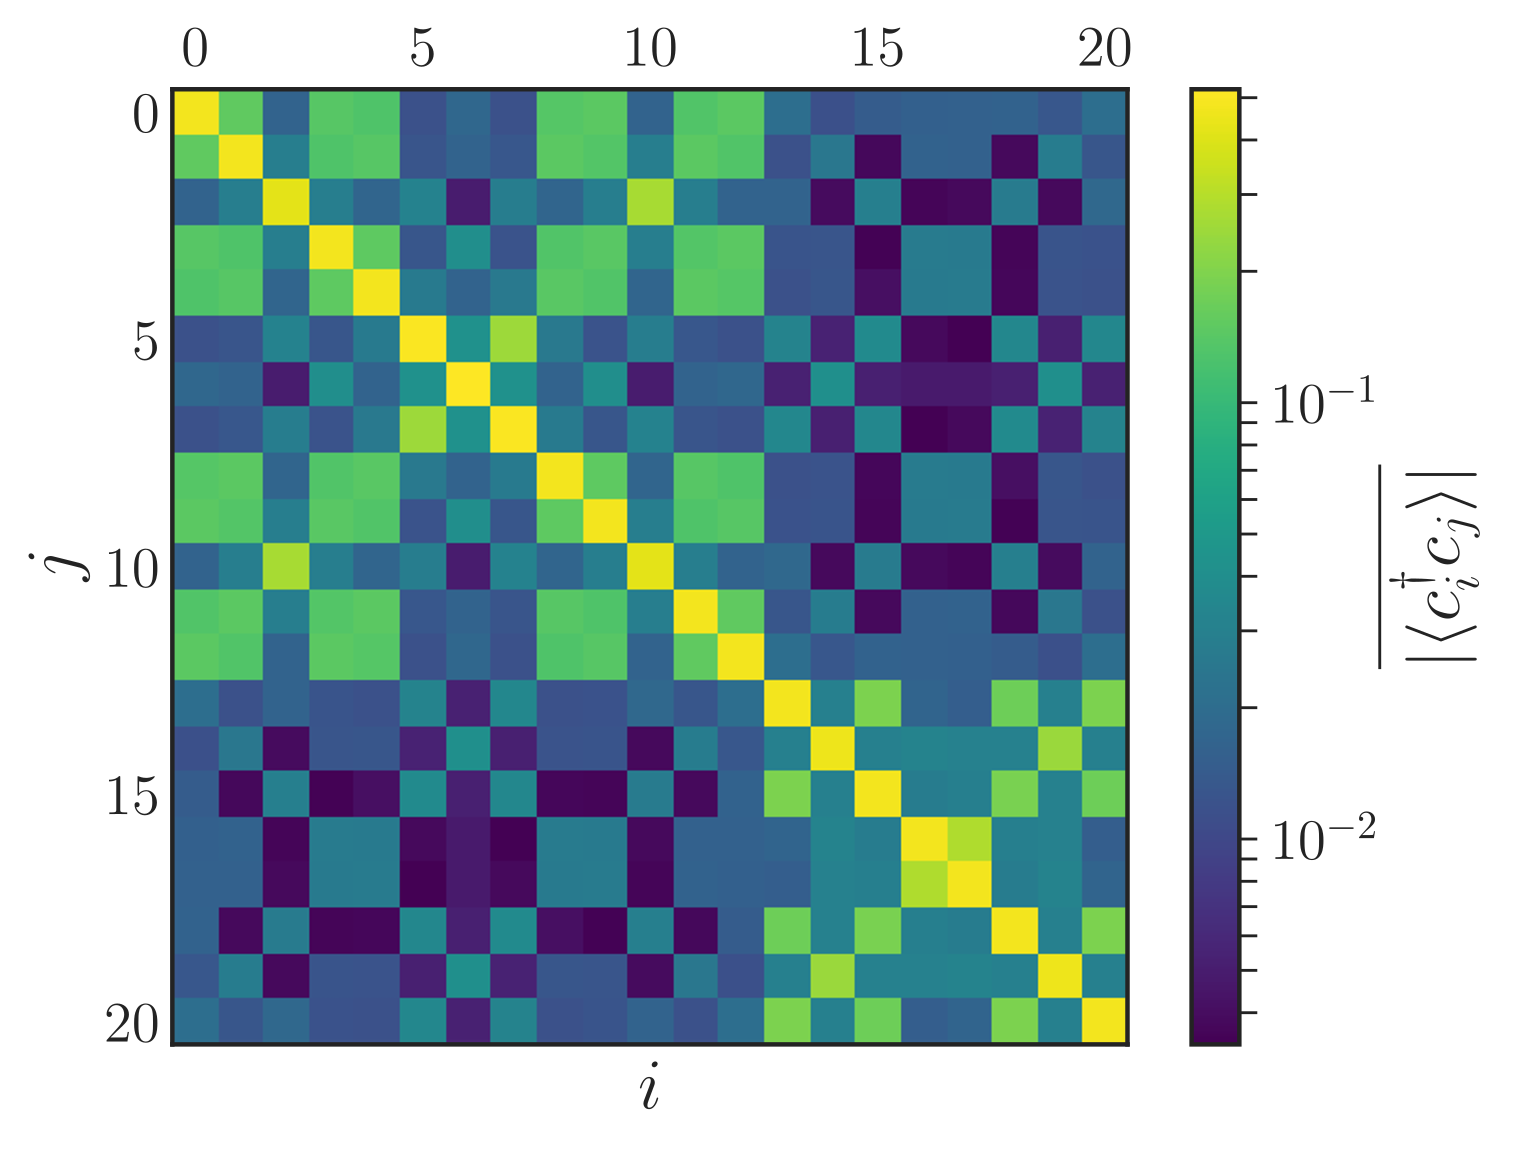
\includegraphics[width=0.8\textwidth]{img/3_Fibonacci/density_matrix_L21_h3}

{\footnotesize Correlations of highly excited states [Macé \emph{et al} 19]}
\end{column}
\end{columns}
\end{frame}

\begin{frame}{Free fermions entanglement}
\begin{block}{Entanglement entropy $S(\psi)$: a many-body \textbf{locality} probe}
\begin{itemize}
	\item $S(\psi) = \#\{\text{bits of information recoverable by local measurements}\}$
	\item $S(\psi)$ large: extended (entangled) state, $S(\psi)$ small: localized state.
\end{itemize}
\end{block}
%%%%%%%%%
\begin{columns}
\begin{column}{0.4\textwidth}
\centering
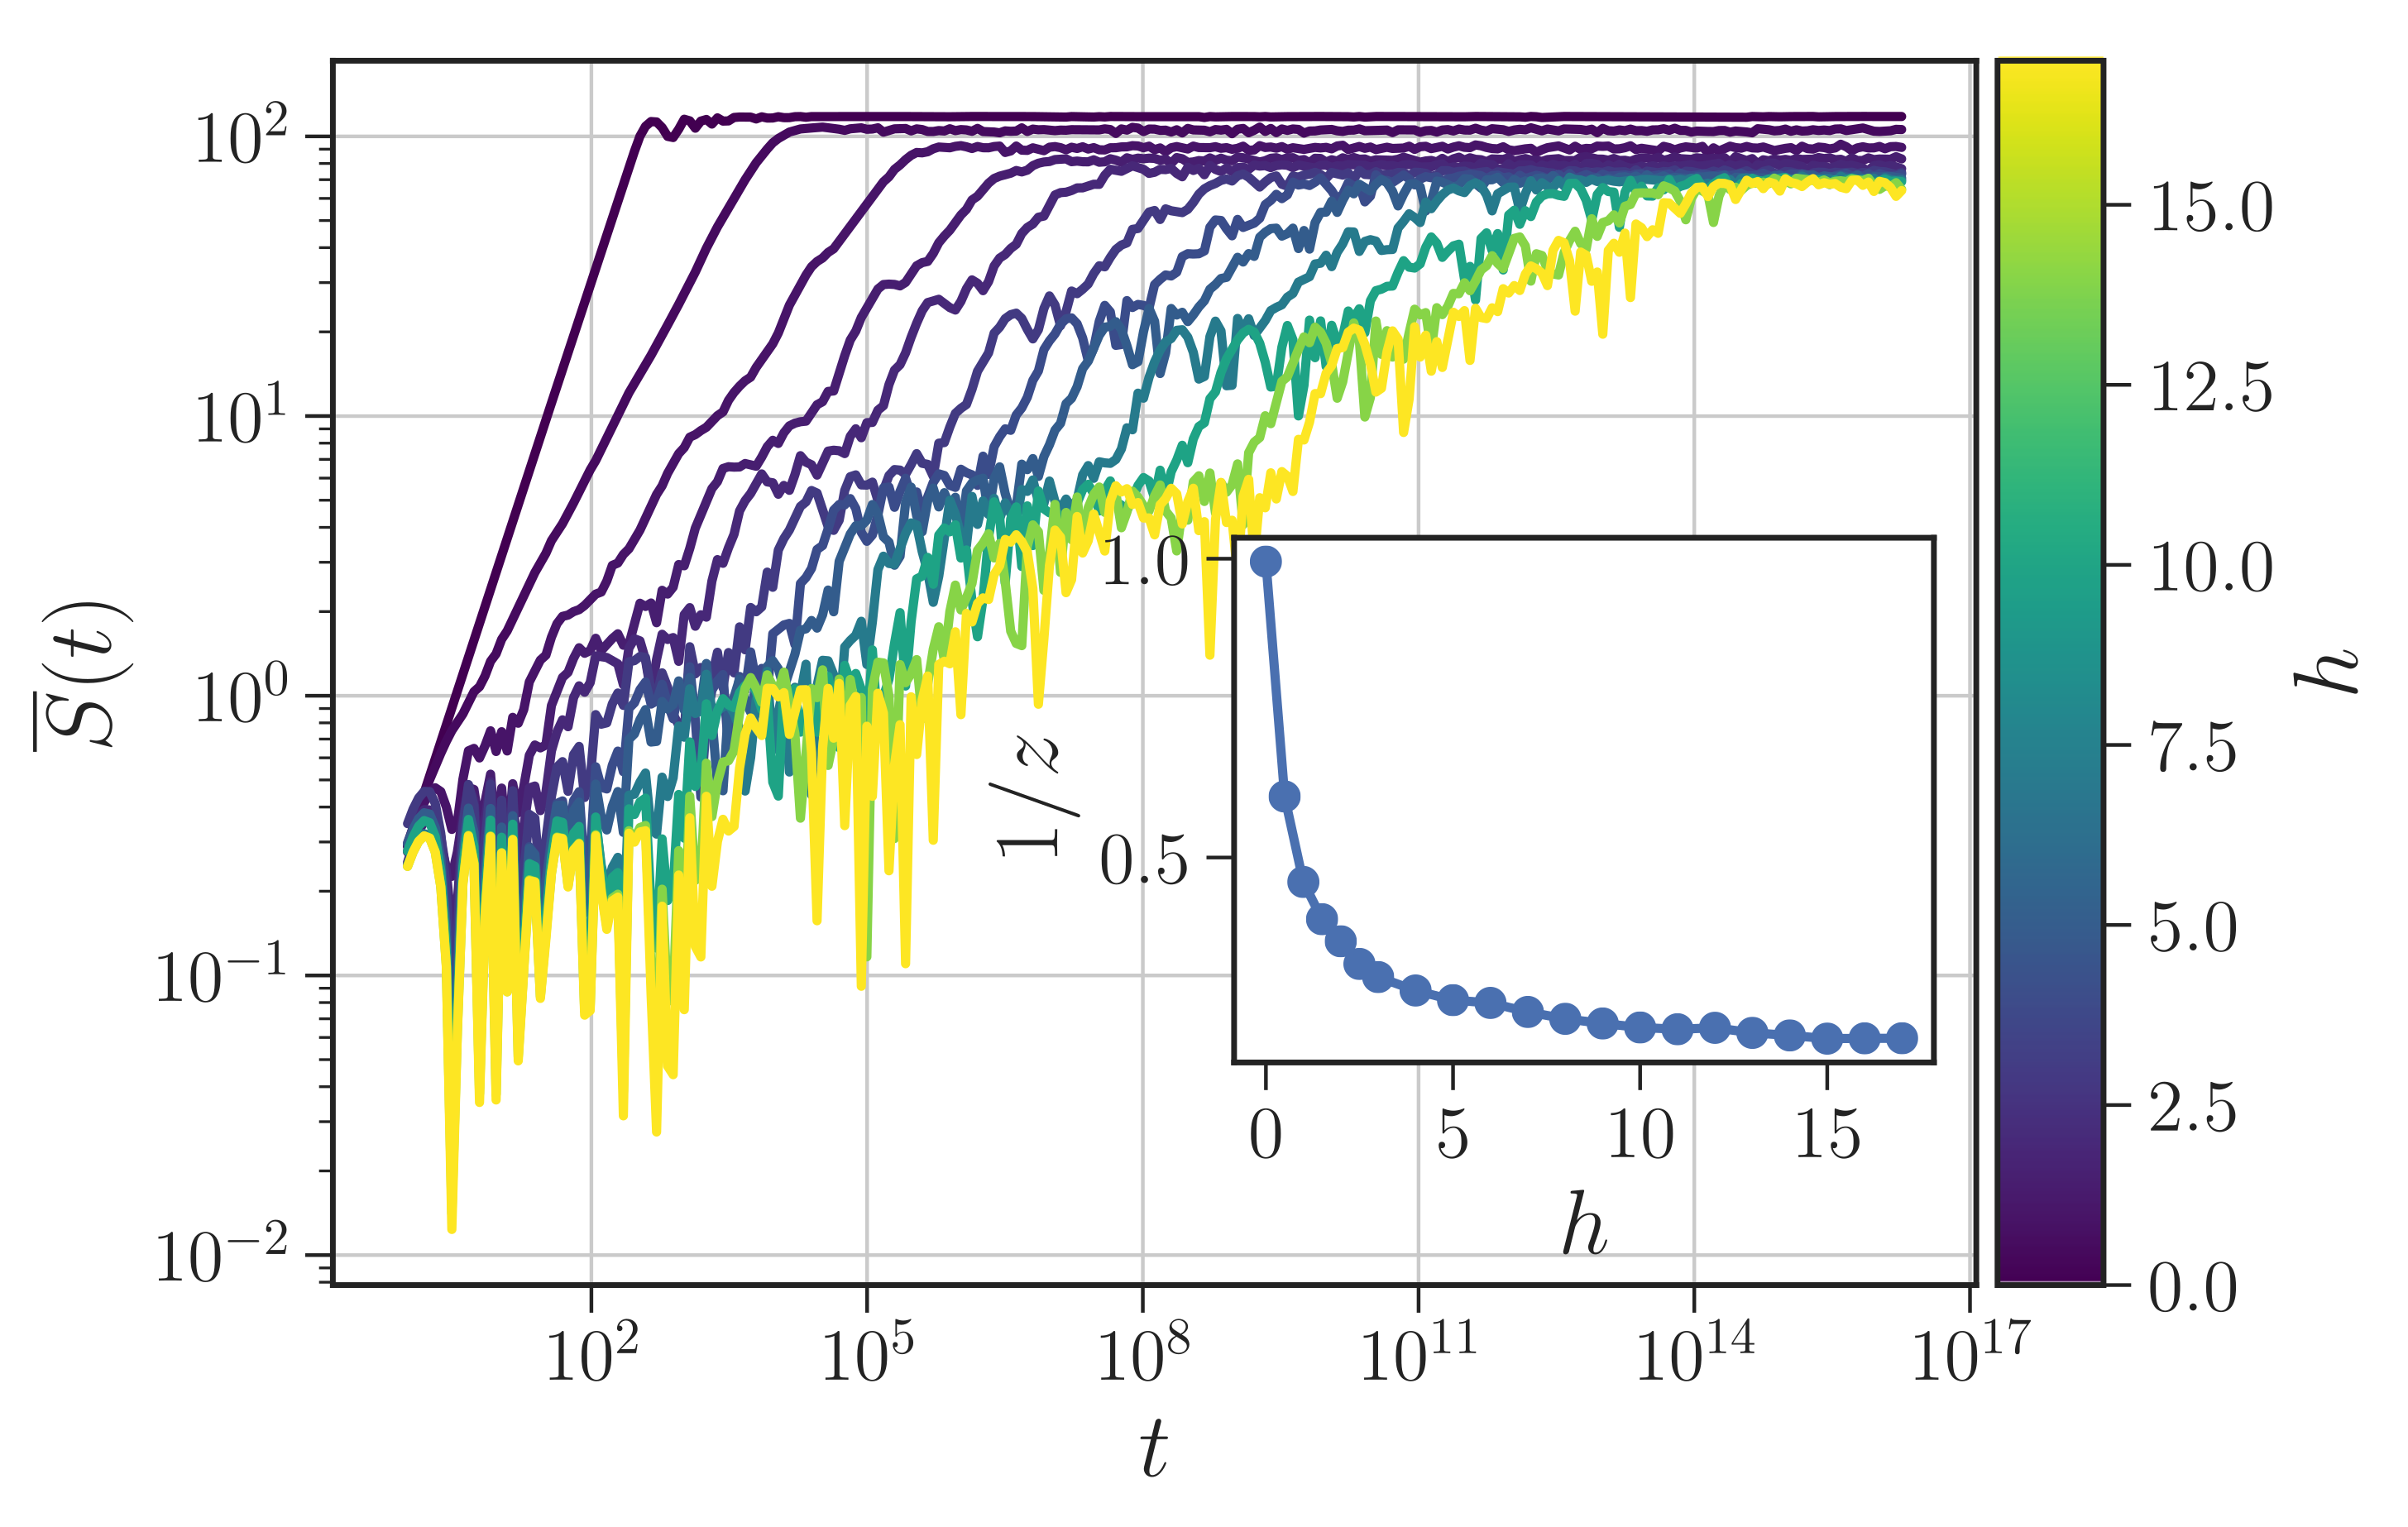
\includegraphics[width=\textwidth]{img/3_Fibonacci/free_fermions_entanglement_inset_coefficients}
{\footnotesize Entanglement growth starting from localized fermions [Macé \emph{et al} 19]}
\end{column}
%%%%%%%%%%%
\begin{column}{0.6\textwidth}
Fibonacci fermions: \textbf{anomalous} growth

$S(t) \sim t^{\frac{1}{z}},~z > 1$

Compare with:
\begin{itemize}
	\item Periodic system: $z=1$ (ballistic growth),
	\item Disordered system: $z \to \infty$ (no growth).
\end{itemize}
\begin{block}{\textbf{Conclusion}}
Anomalous, intermediate prop.\, even at high energy.
\end{block}
\end{column}
\end{columns}
\end{frame}

\section{Interacting Fibonacci chain}
\subsection{Dummy}
\begin{frame}{The ETH/MBL transition: 1) spectral properties}
\begin{columns}
\begin{column}{0.5\textwidth}
Gap ratios {\footnotesize [Oganesian, Huse]}
\[
	r_n = \min\left(\frac{g_{n+1}}{g_n}, \frac{g_n}{g_{n+1}}\right)
\]
\begin{itemize}
	\item \textcolor{comp}{ETH: random matrix-like spectrum}
	$\overline{r}_\text{ETH} \simeq 0.53$
	\item \textcolor{BostonBlue}{MBL: independant levels}
	
	$\overline{r}_\text{MBL} \simeq 0.39$
\end{itemize}
\end{column}
%%%%%%%%%%%%%%%
\begin{column}{0.5\textwidth}
\centering
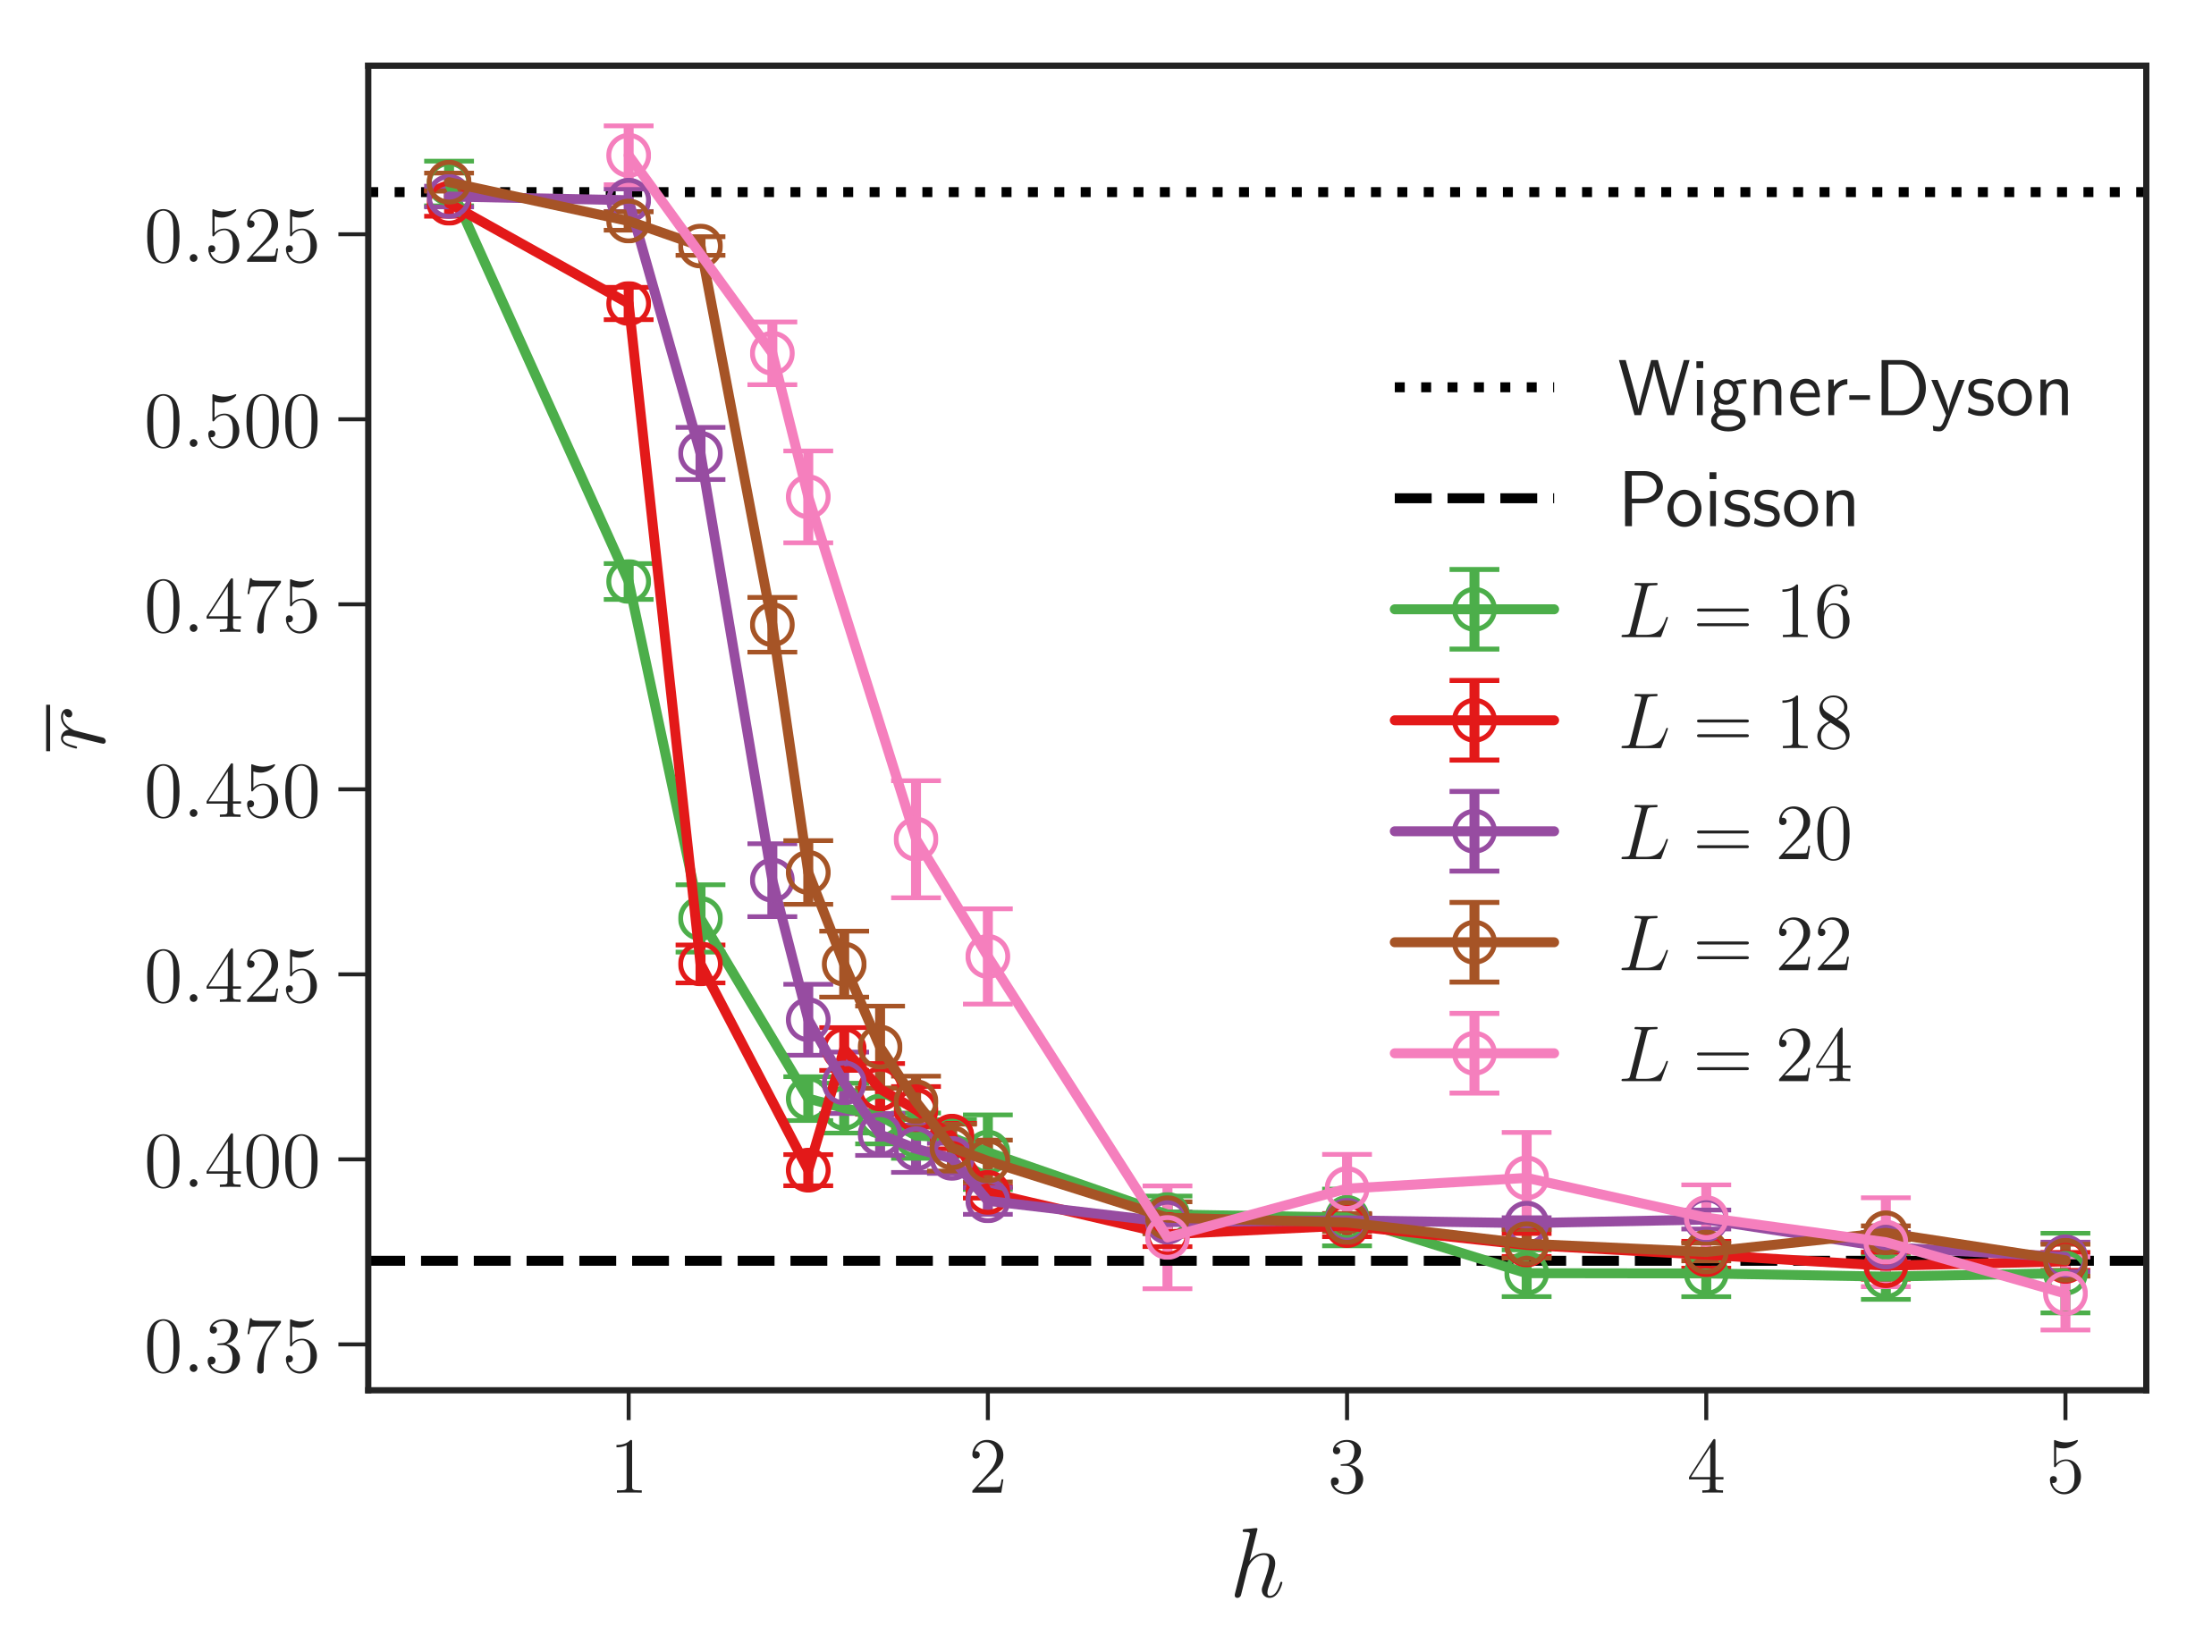
\includegraphics[width=0.9\textwidth]{img/3_Fibonacci/rgap}

Compatible with \textbf{ETH/MBL transition}, $h^* \simeq 2.5$.
\end{column}
\end{columns}
\end{frame}

\begin{frame}{The ETH/MBL transition: 2) Entanglement}
\begin{columns}
\begin{column}{0.5\textwidth}
Entanglement entropy:
\begin{itemize}
	\item \textcolor{comp}{ETH: coincides with thermodynamic entropy: \textbf{extensive}}
	
	$\overline{S}_\text{ETH} \simeq L$
	\item \textcolor{BostonBlue}{MBL: \textbf{sub-extensive}}
	
	$\overline{S}_\text{MBL}/L \to 0$
\end{itemize}
\end{column}
%%%%%%%%%%%%%%%
\begin{column}{0.5\textwidth}
\centering
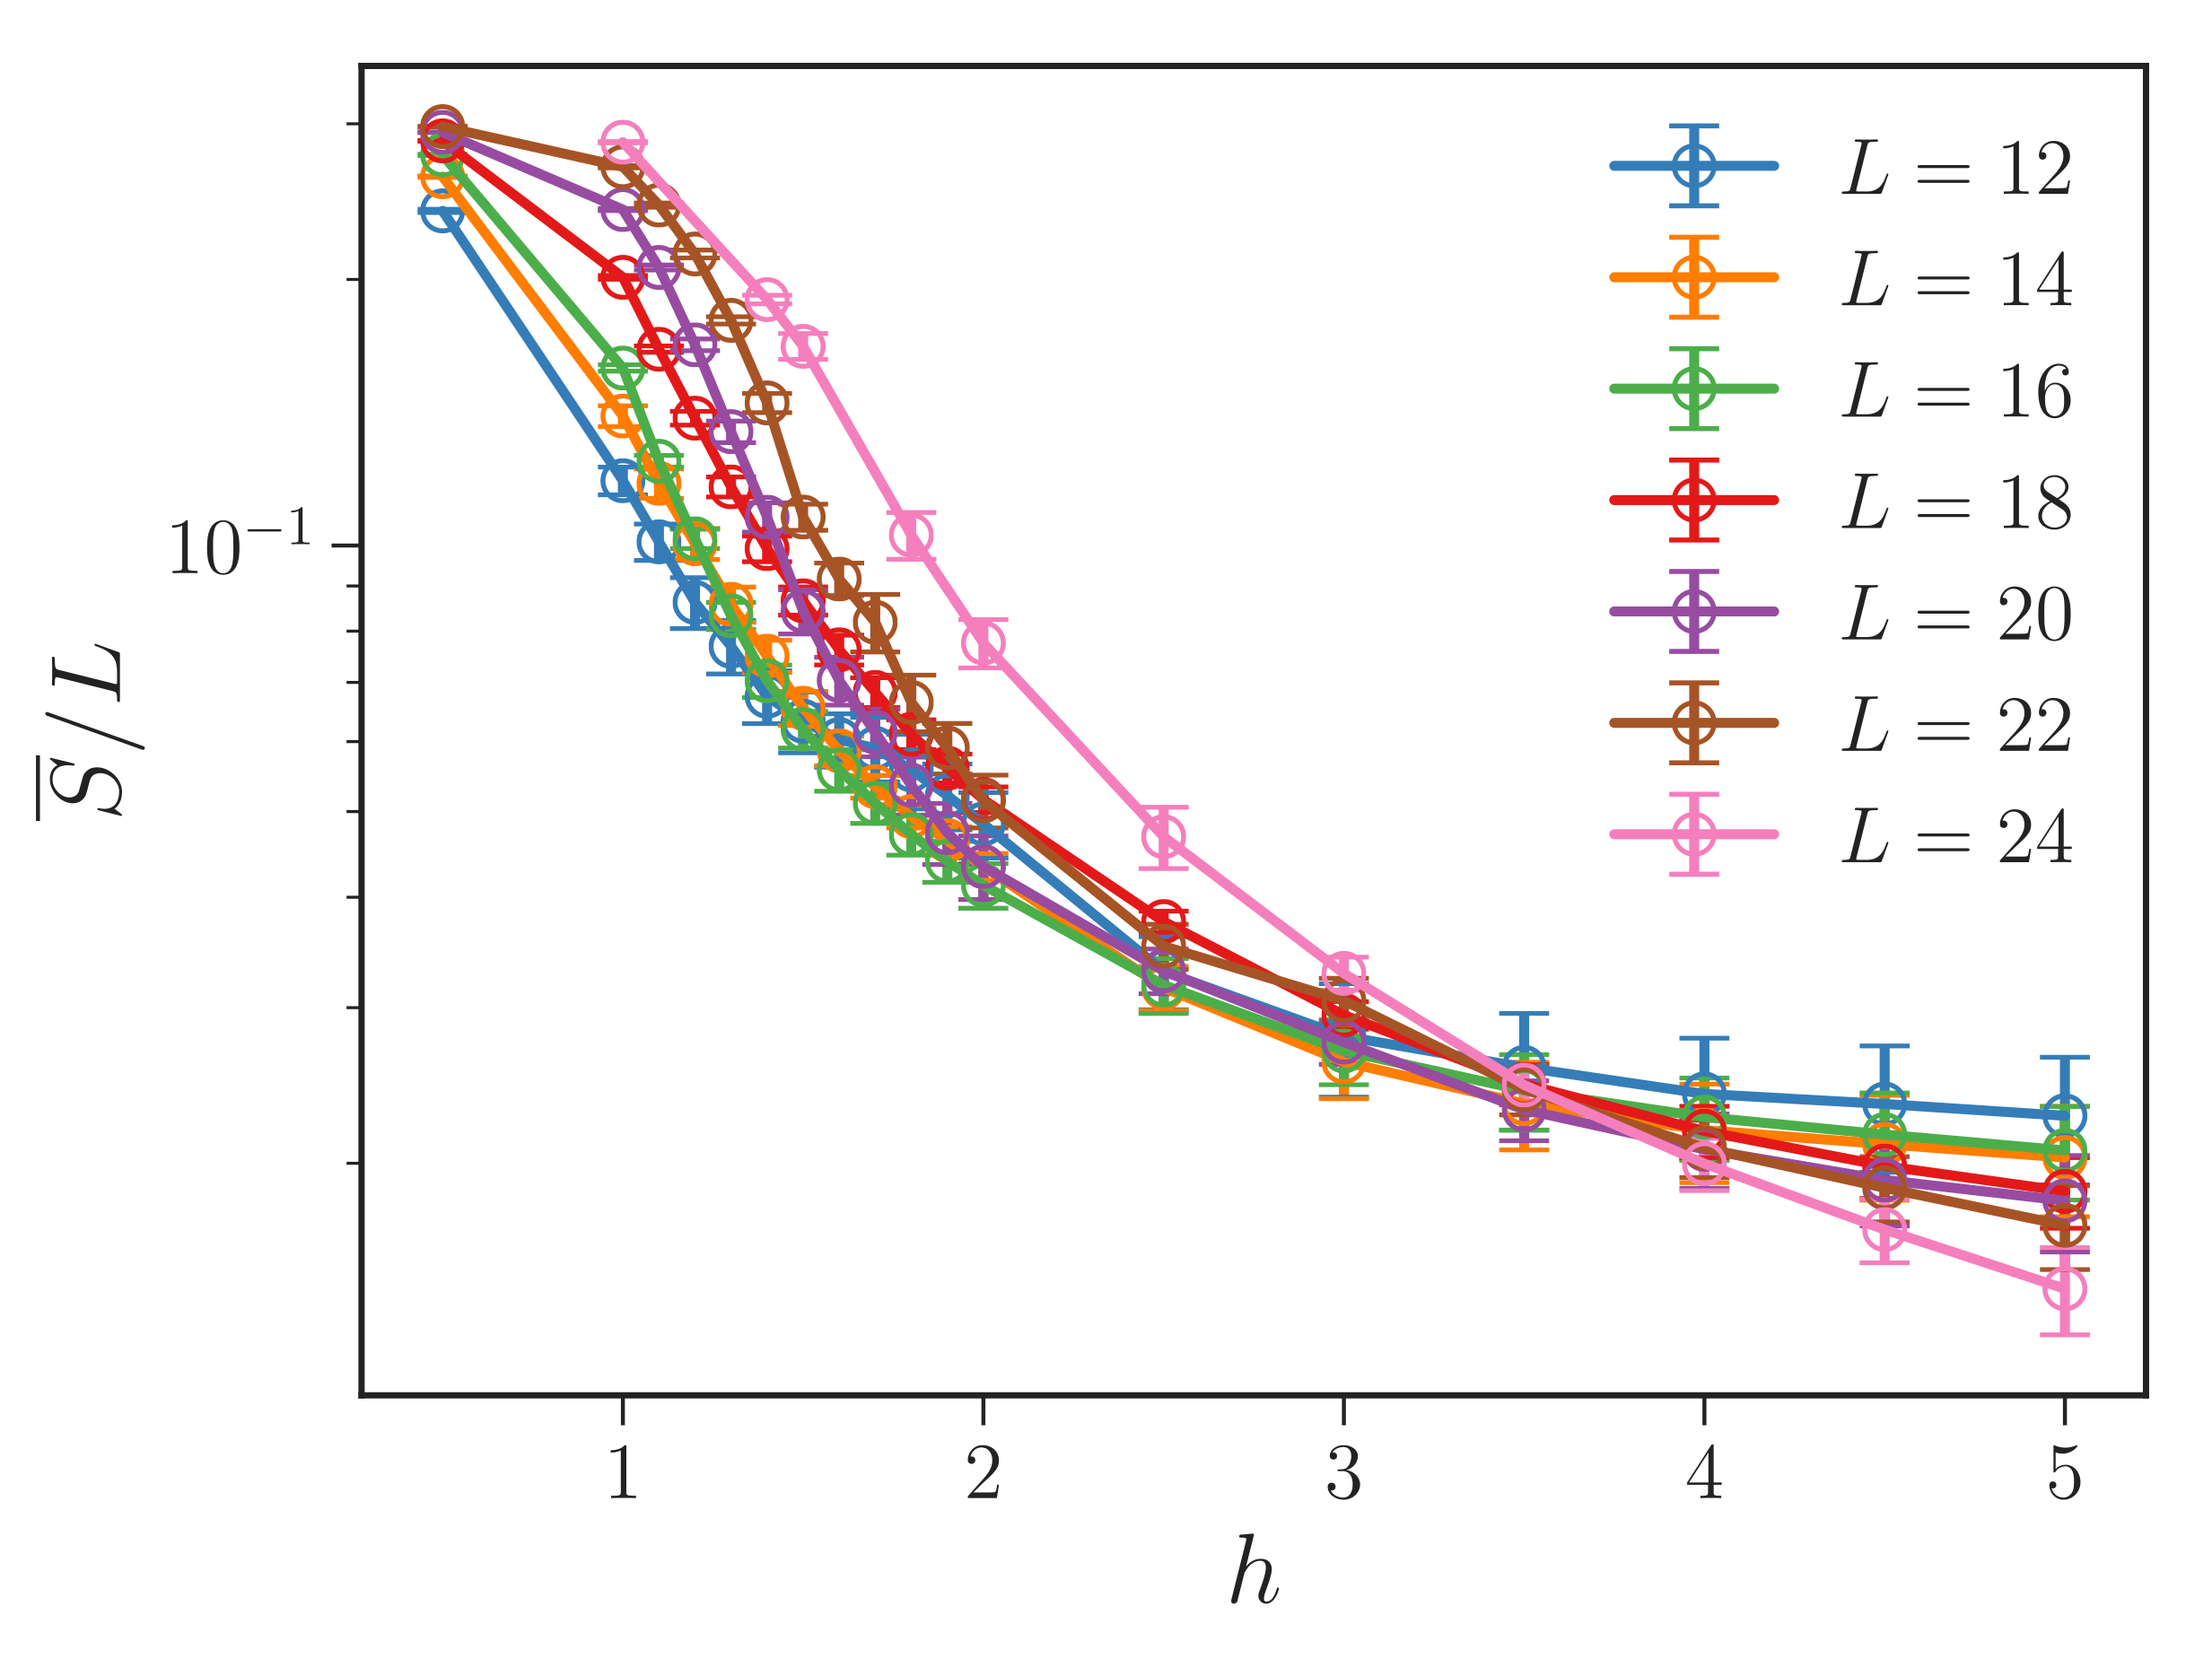
\includegraphics[width=0.9\textwidth]{img/3_Fibonacci/entropy}

Compatible with \textbf{ETH/MBL transition}, $h^* \simeq 3.5$.
\end{column}
\end{columns}
\end{frame}

\begin{frame}{The ETH/MBL transition: 3) Local observables}
Expect: \textcolor{comp}{$\langle n_i \rangle_\text{ETH} = \frac{1}{2}$}, \textcolor{BostonBlue}{$\langle n_i \rangle_\text{MBL} \simeq 0 \text{ or } 1$}.
\begin{columns}
\begin{column}{0.33\textwidth}
\centering
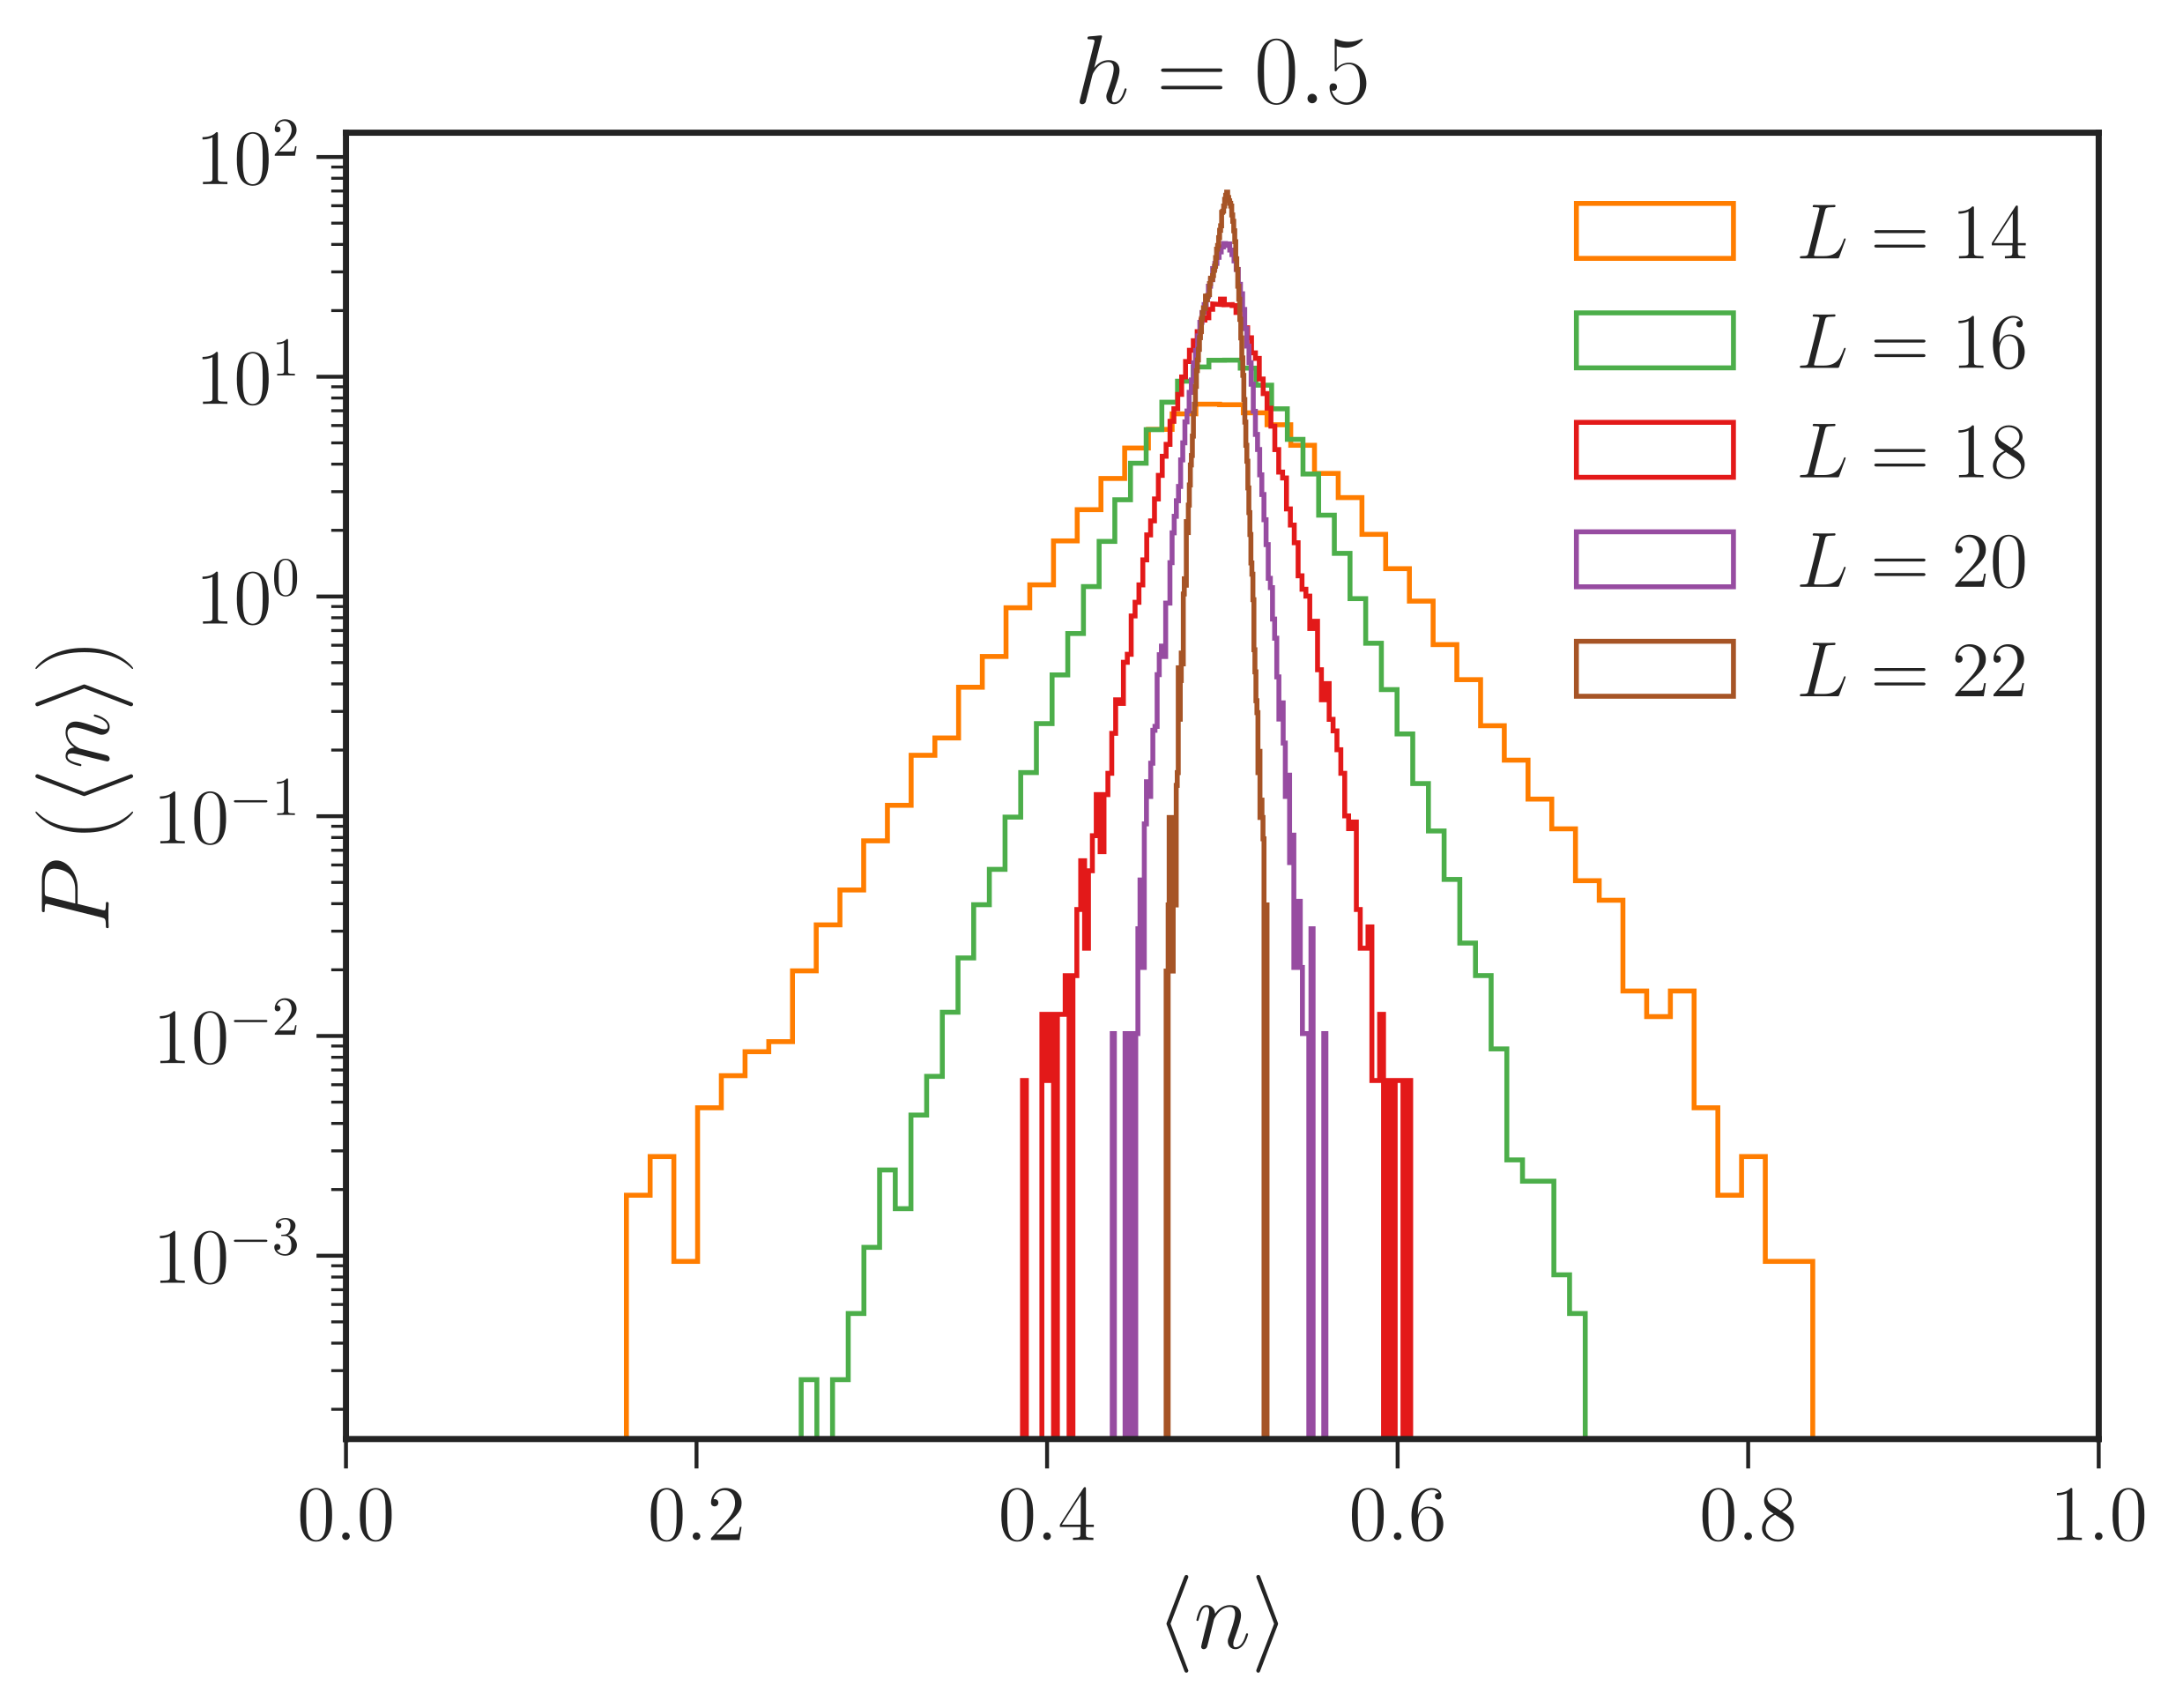
\includegraphics[width=\textwidth]{img/3_Fibonacci/sz_ETH}
{\footnotesize ETH Fibonacci}
\end{column}
%%%%%%%%%%
\begin{column}{0.33\textwidth}
\centering
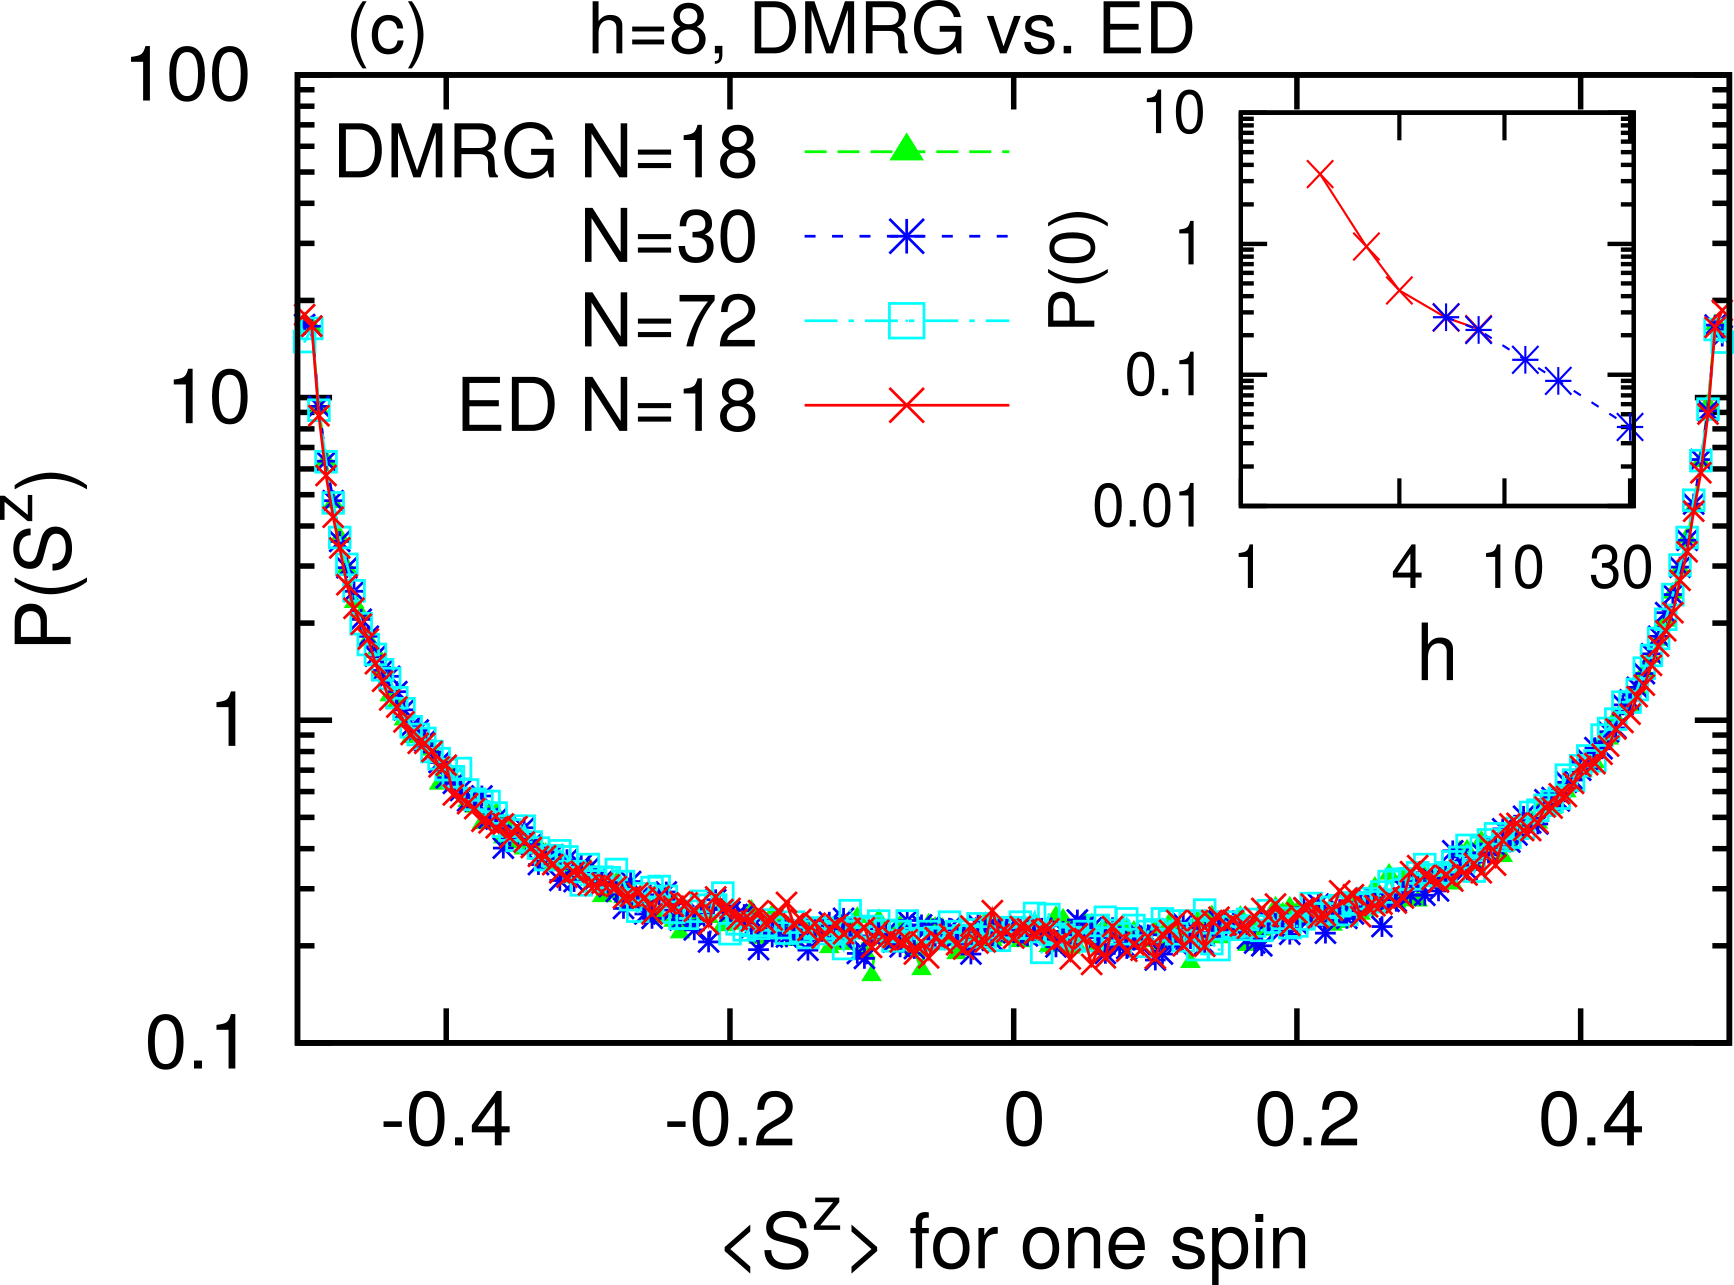
\includegraphics[width=\textwidth]{img/3_Fibonacci/surface768}
{\footnotesize MBL random [Lim, Sheng 15]}
\end{column}
%%%%%%%%%%
\begin{column}{0.33\textwidth}
\centering
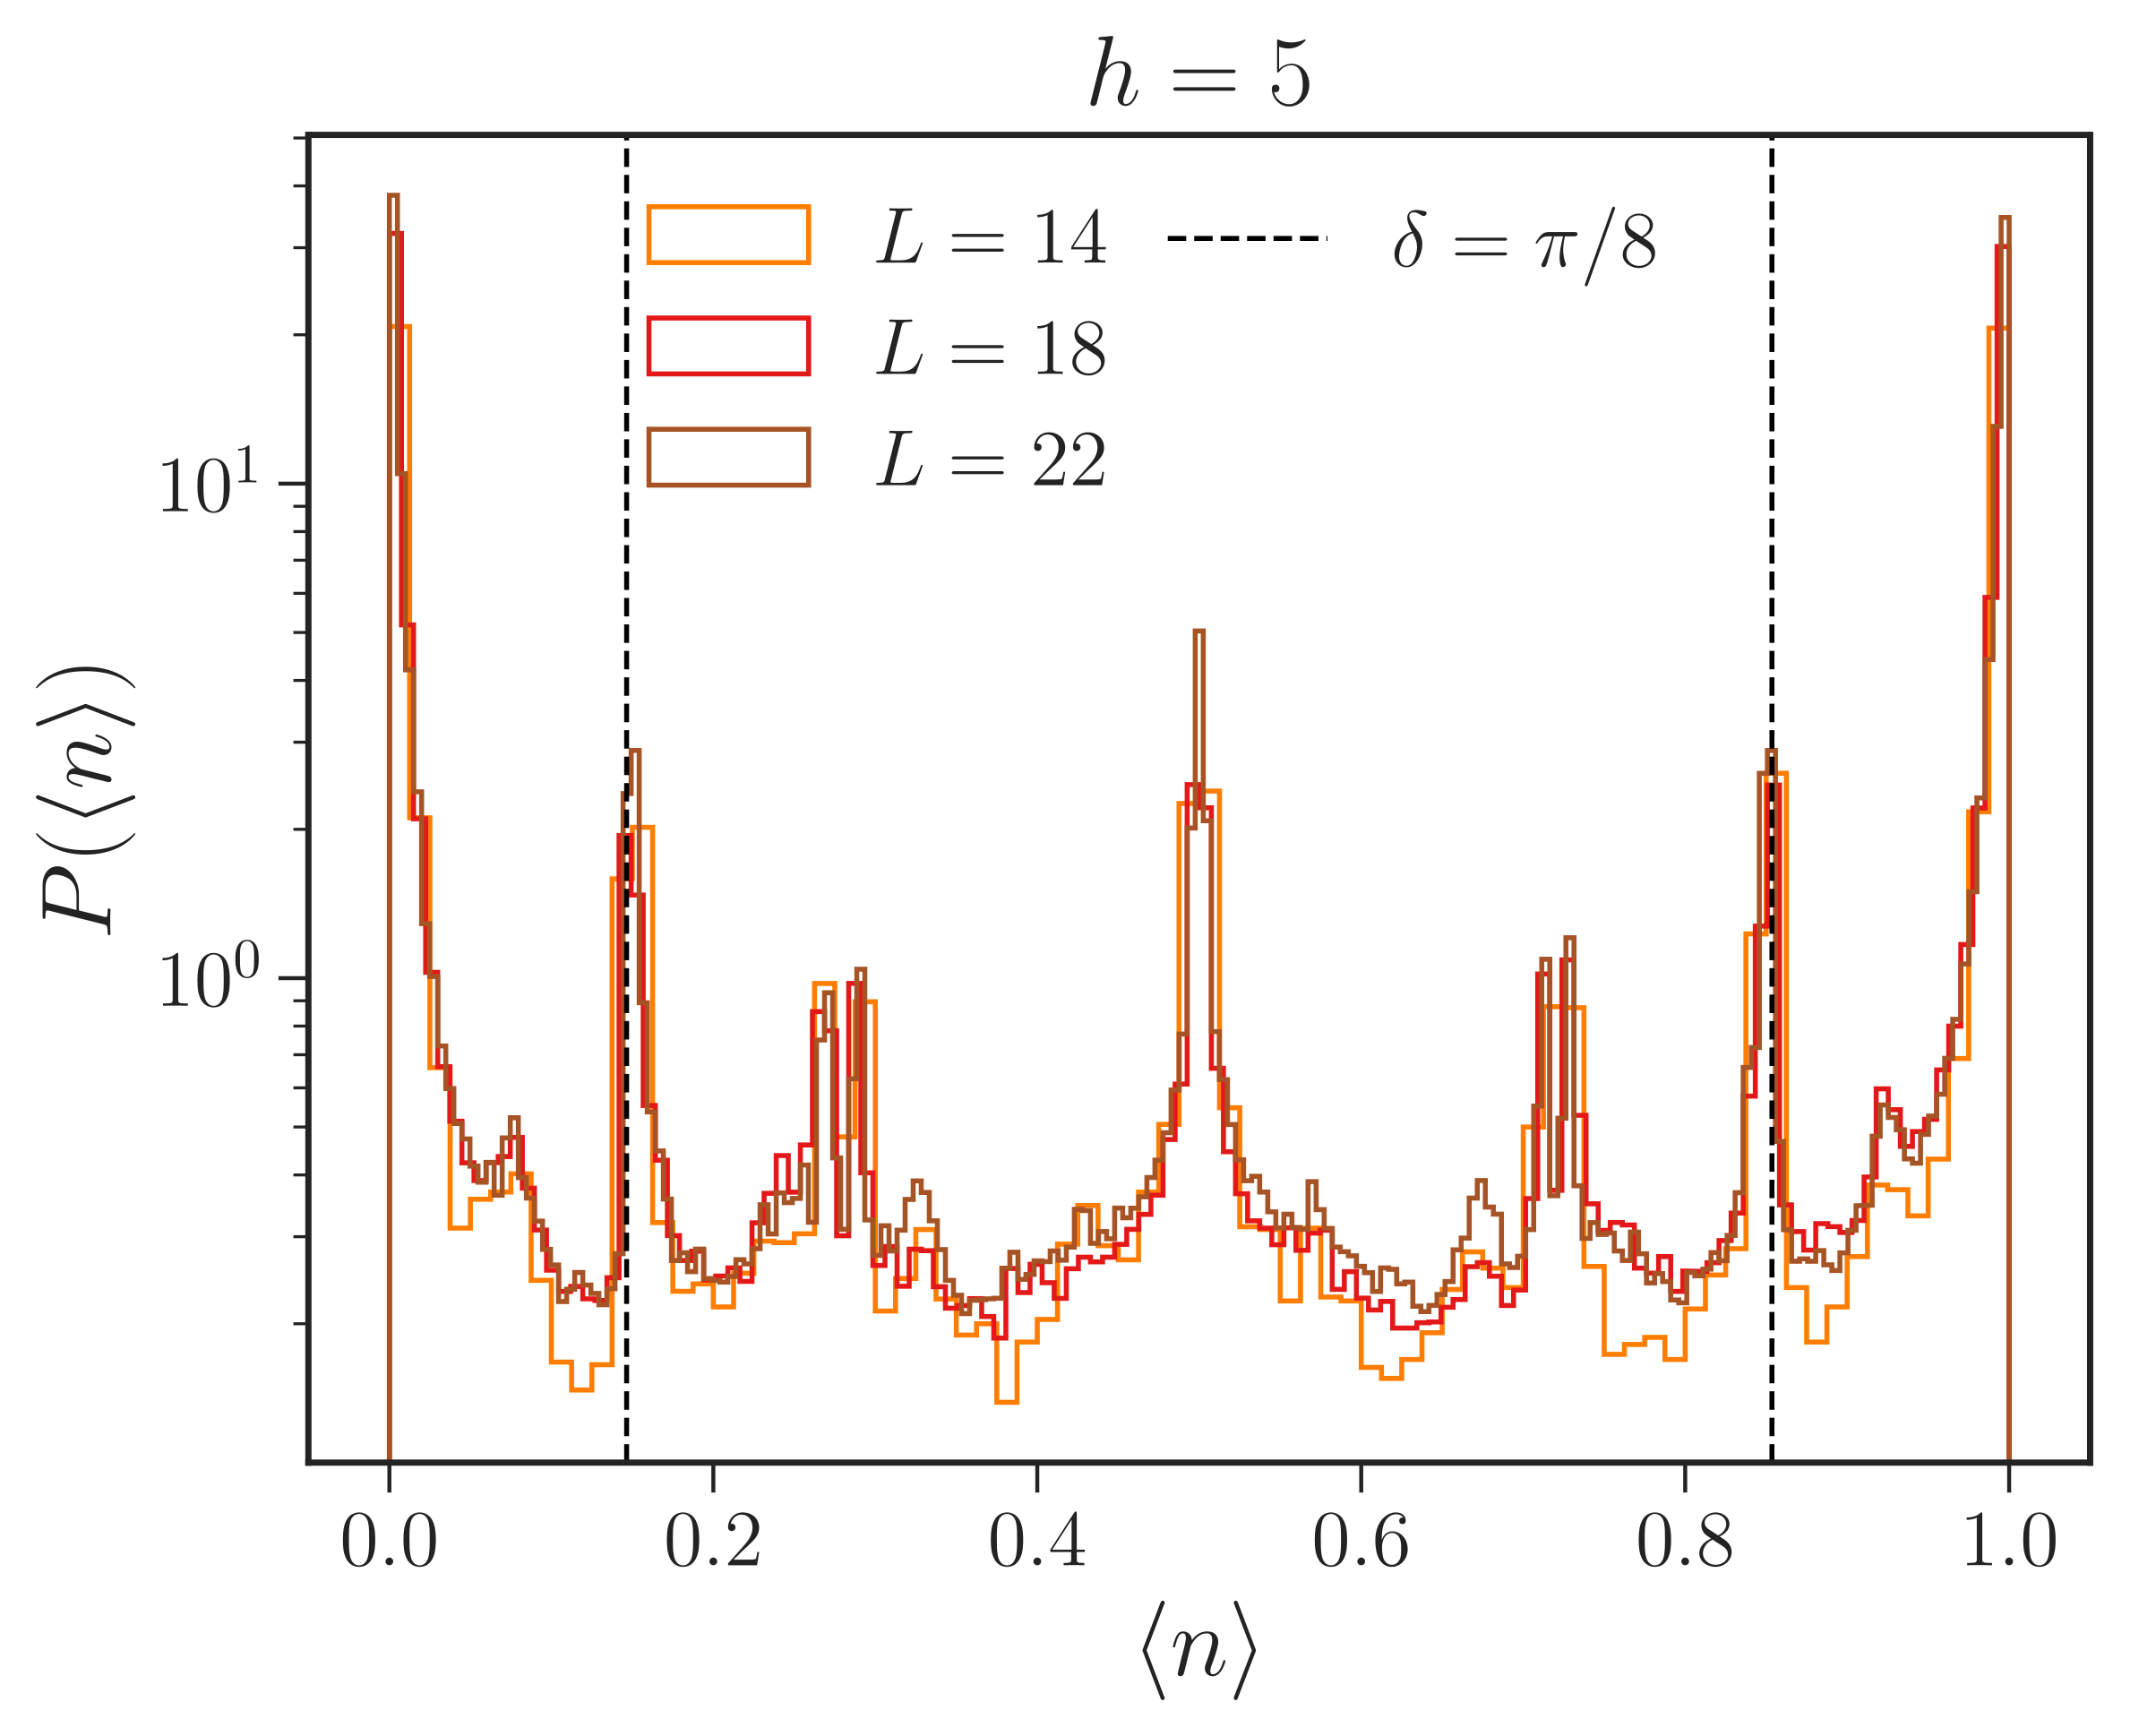
\includegraphics[width=\textwidth]{img/3_Fibonacci/sz_MBL}
{\footnotesize MBL Fibonacci}
\end{column}
%%%%%%%%%%
\end{columns}
~\\
~\\

Fibonacci MBL: \textbf{extra structure} $\to$ link with QP geometry?
\end{frame}

\begin{frame}{Fibonacci MBL: local entanglement}
\begin{columns}
\begin{column}{0.5\textwidth}
\centering
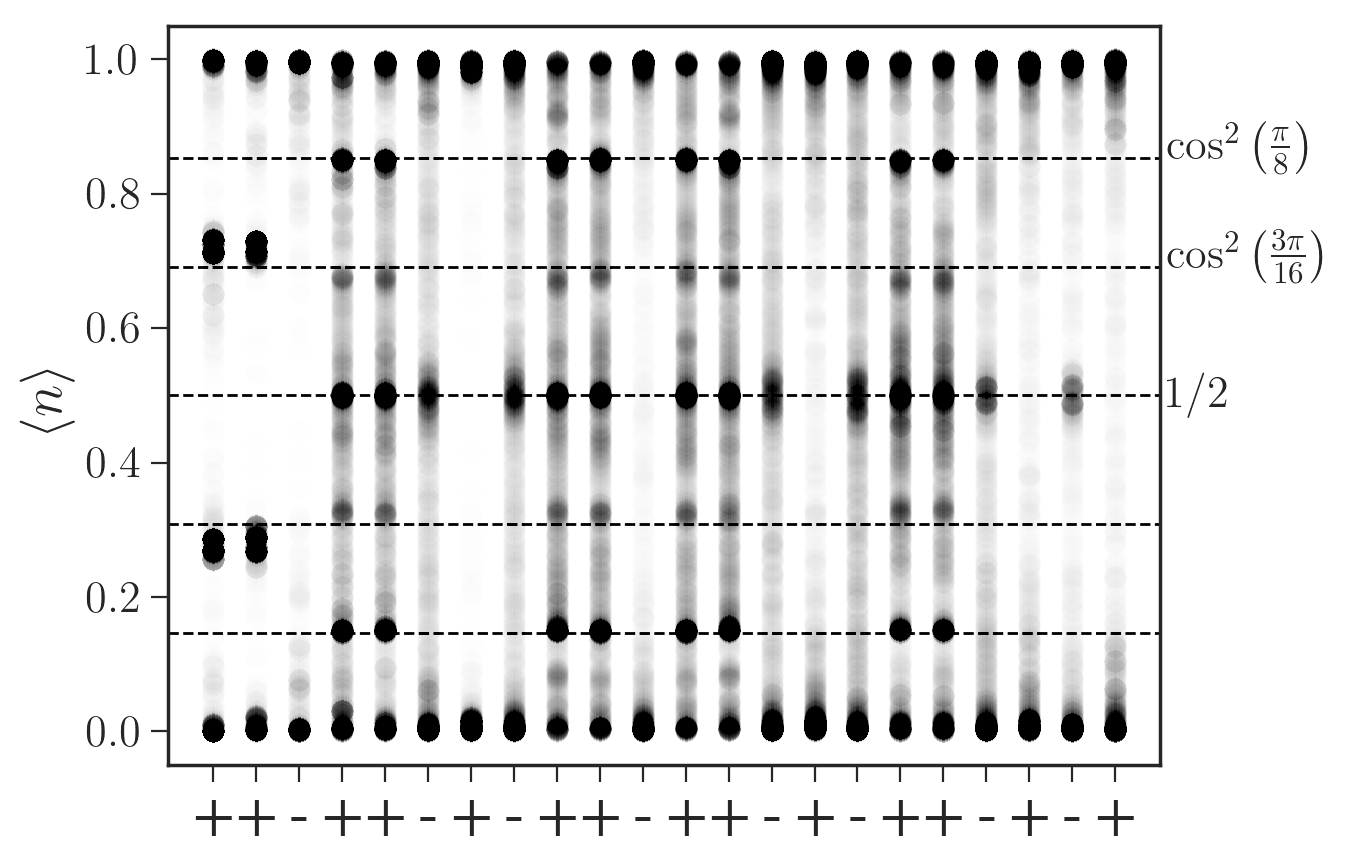
\includegraphics[width=0.8\textwidth]{img/3_Fibonacci/realspace_sz_L22_h5_shift1}
\end{column}
%%%%%%%%%%%%
\begin{column}{0.5\textwidth}
Density peaks on \textbf{AA pairs}

$\to$ 4 sites toy model BAAB

$\to$ locally entangled states

$\ket{\psi} = \cos \delta \ket{01} \pm \sin \delta \ket{10}$

with $\delta = 0,~\frac{\pi}{4},~\frac{\pi}{8}$.
\end{column}
\end{columns}
%%%%%%%%%%%%%%%%%%%%%%%%%%%%%%%
\begin{columns}
\begin{column}{0.33\textwidth}
\centering
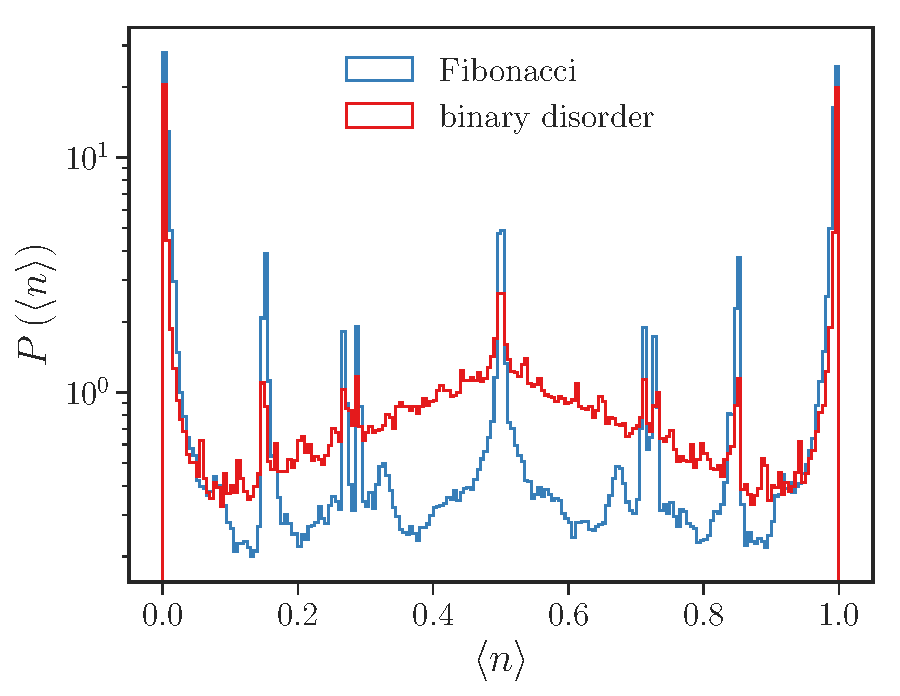
\includegraphics[width=0.8\textwidth]{img/3_Fibonacci/local_observable_fibo_shuffle_p_8_h_5_L_22}
\end{column}
%%%%%%%%%%%%
\begin{column}{0.33\textwidth}
Peak ingredients:
\begin{itemize}
	\item \textbf{Binary} modulation A/B
	\item \textbf{Correlated} modulation (Fibonacci)
\end{itemize}
\end{column}
%%%%%%%%%%%%
\begin{column}{0.33\textwidth}
\centering
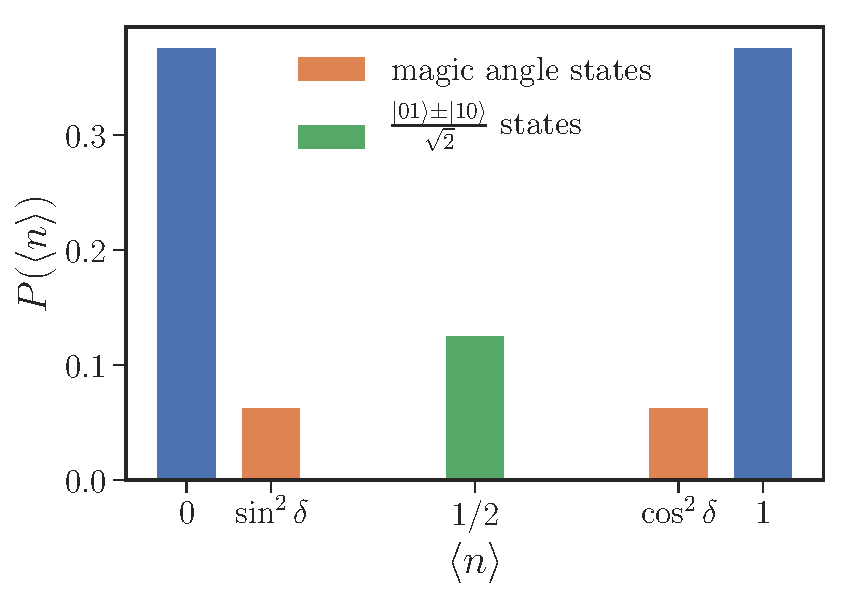
\includegraphics[width=0.8\textwidth]{img/3_Fibonacci/sz_perturbation_theory}
\end{column}
\end{columns}
\end{frame}

\begin{frame}{Dynamics: Imbalance}
\begin{columns}
\begin{column}{0.5\textwidth}
Imbalance experiment:
\begin{itemize}
	\item $\ket{\psi(t=0)}$: high energy product state
	\item Imbalance: \textbf{distance} from initial state
	
	$I(t) = \frac{4}{L}\sum_i \left\langle \left(n_i(t) - \frac{1}{2}\right)\left(n_i(0) - \frac{1}{2}\right) \right\rangle$
\end{itemize}

Properties:
\begin{itemize}
	\item \textcolor{comp}{ETH: power-law decay} $I(t) \sim t^{-\zeta}$
	\item \textcolor{BostonBlue}{MBL: saturation} $I(t\to \infty) = \text{cst} > 0$ 
	
	$\to$ \textbf{memory} of the initial state
	
	{\footnotesize [Luitz \emph{et at} 15]}
\end{itemize}
\end{column}
%%%%%%%%%%%%%%%%
\begin{column}{0.5\textwidth}
\centering
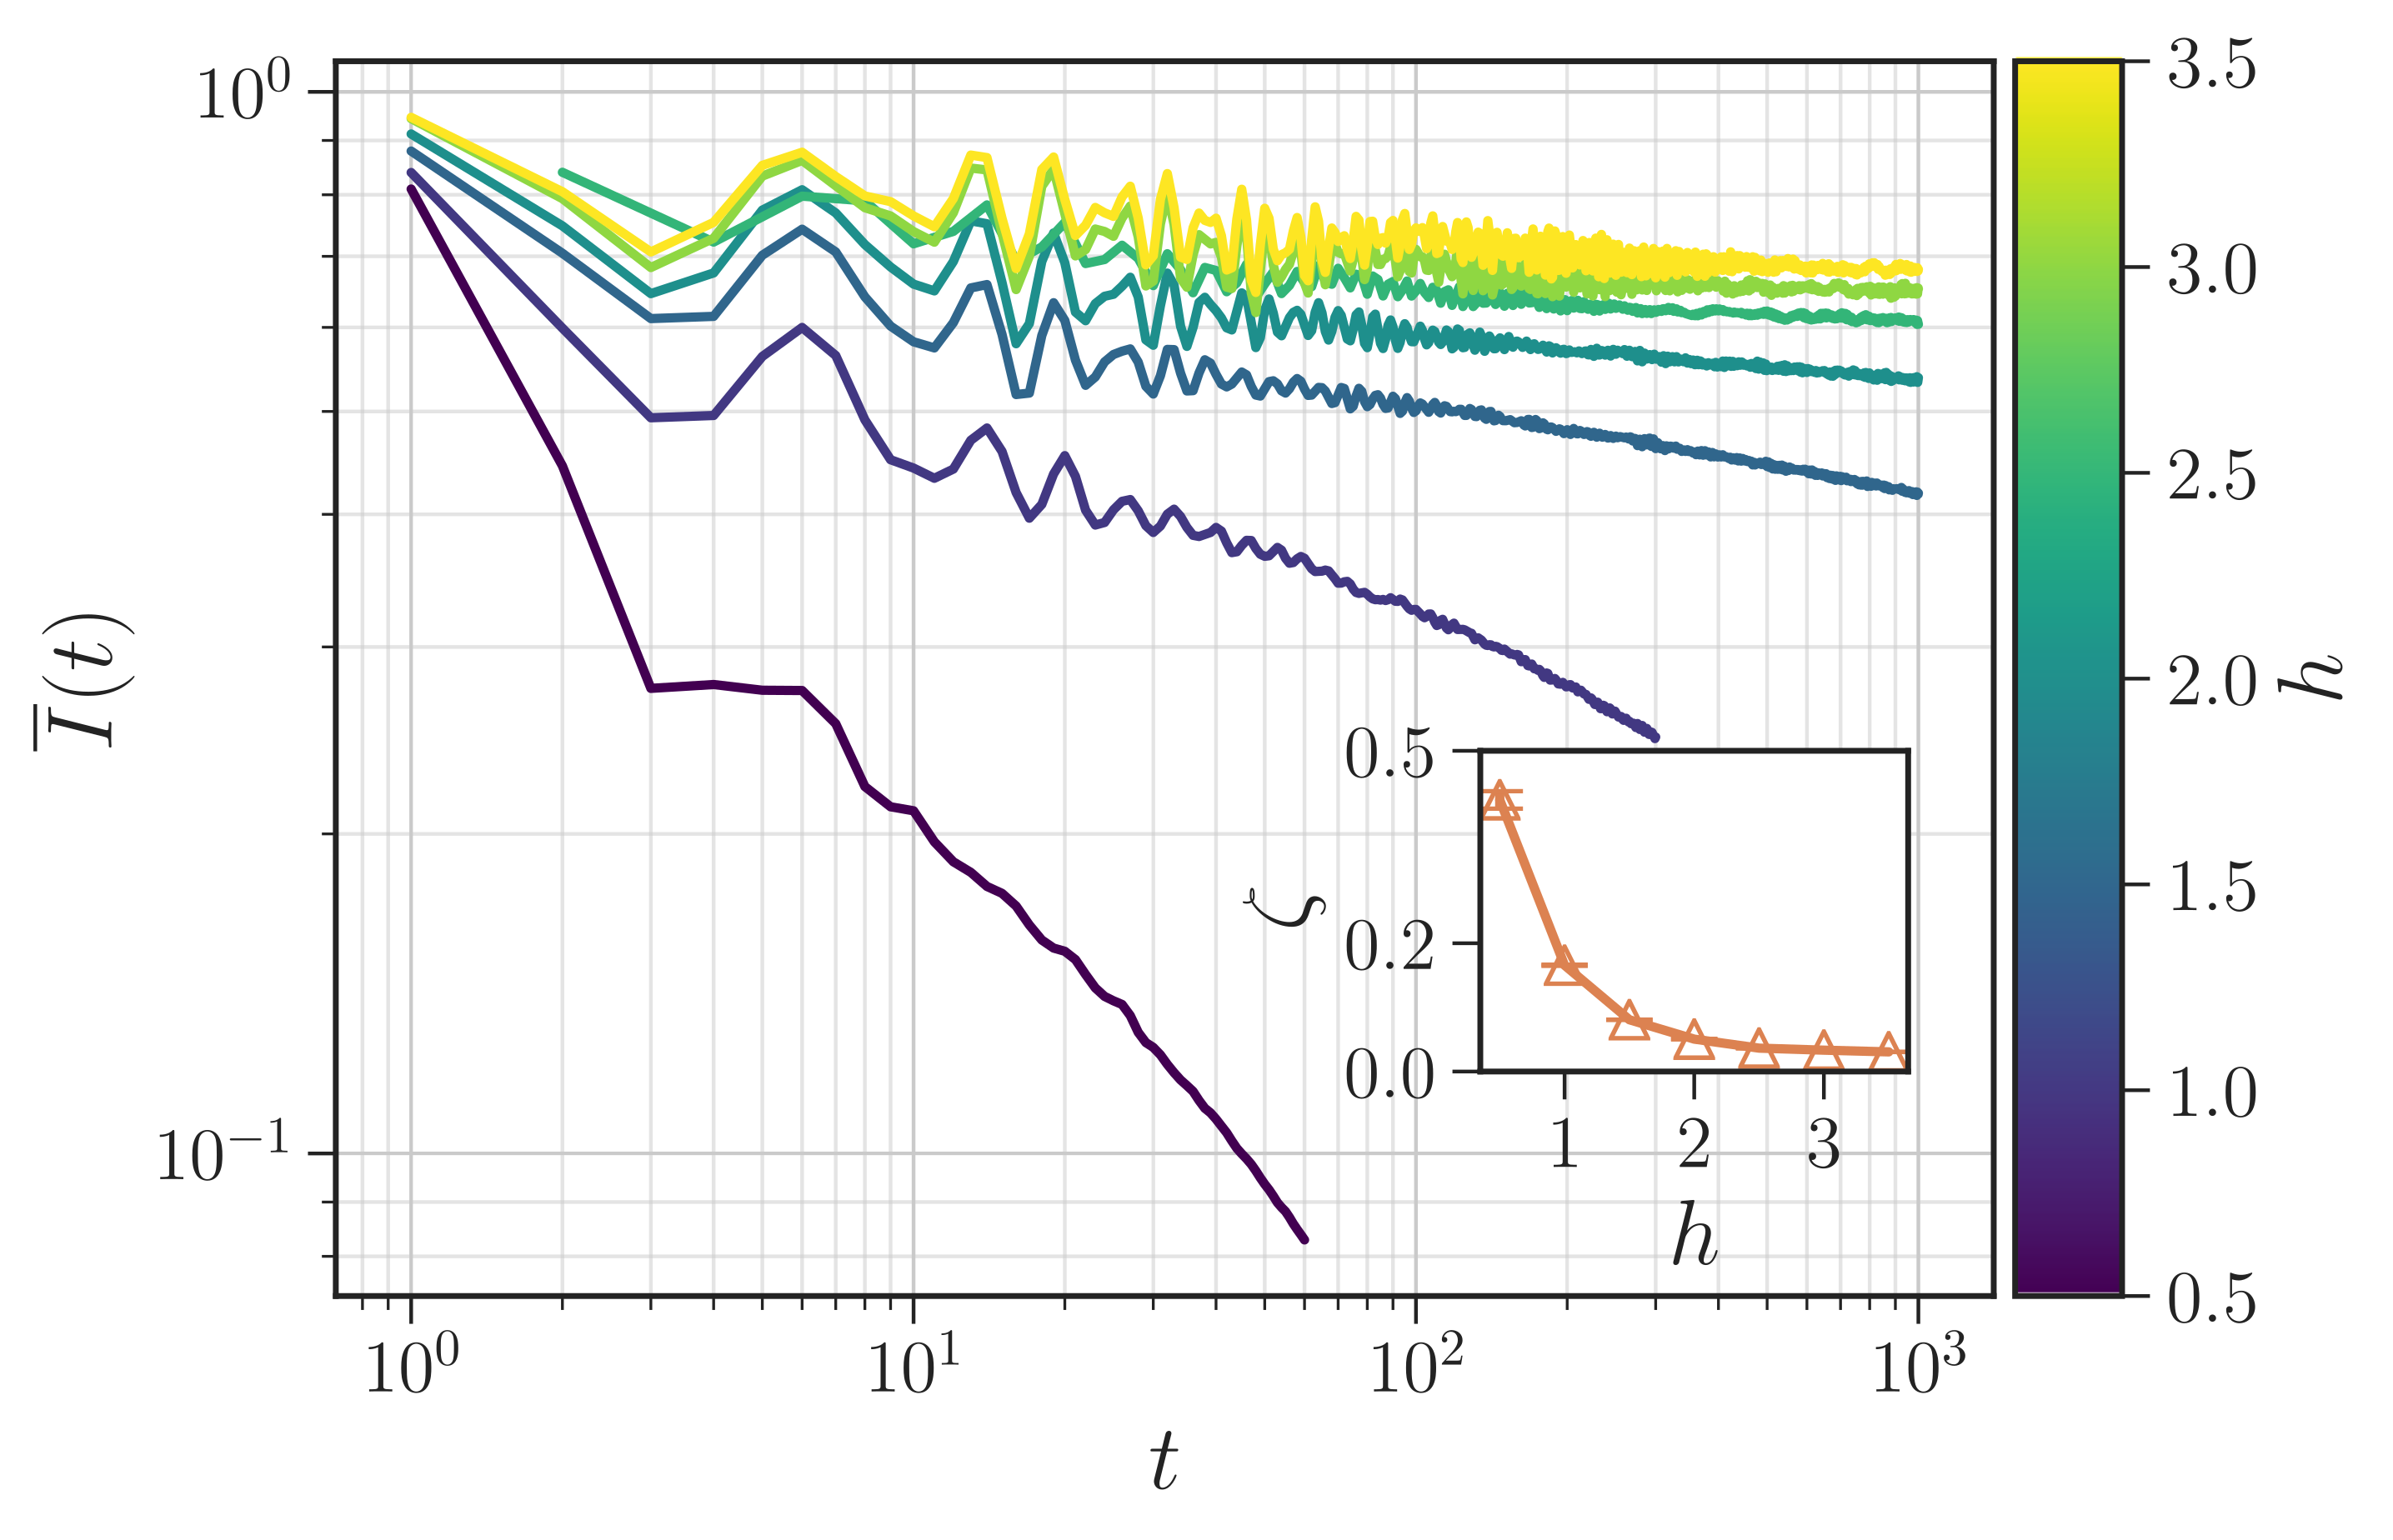
\includegraphics[width=\textwidth]{img/3_Fibonacci/imbalance}

$\zeta(h \geq 2.5) = 0 \to$ MBL phase transition.
\end{column}
%%%%%%%%%%%%%%%%
\end{columns}
\end{frame}

\begin{frame}{Dynamics: entanglement}
\textcolor{comp}{ETH phase}: expect $S(t) \propto t$

Fibonacci: \textbf{anomalous} $S(t) \propto t^{1/z}$, $z > 1$.

\begin{columns}
\begin{column}{0.5\textwidth}
\centering
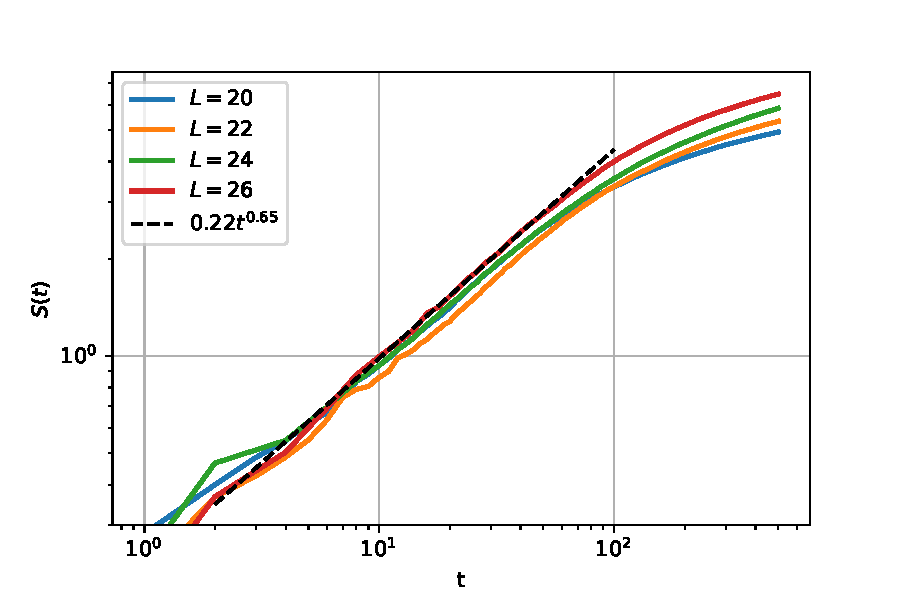
\includegraphics[width=0.8\textwidth]{img/3_Fibonacci/entanglement_scaling_h1_shift0}
\end{column}
%%%%%%%%%%%%%
\begin{column}{0.5\textwidth}
\centering
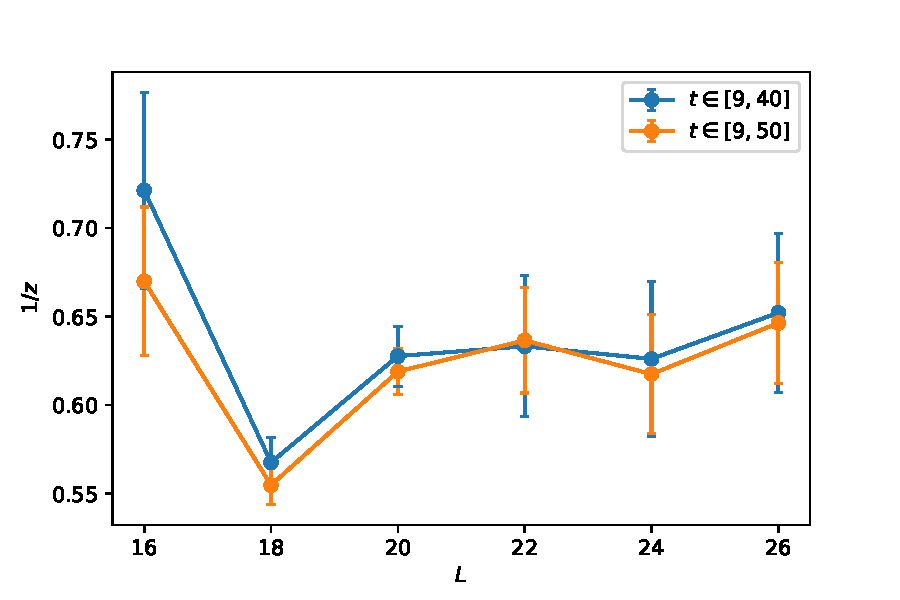
\includegraphics[width=0.8\textwidth]{img/3_Fibonacci/fits_entropy_h1_shift0}
\end{column}
\end{columns}
Usual explanation: \textbf{rare regions} {\footnotesize[Vosk; Potter 15]}

Fibonacci: no rare regions \dots 

Finite size effect? {\footnotesize[Setiawan \emph{et al} 17]}, initial state fluctuations? {\footnotesize[Lüschen \emph{et al} 17]}
\end{frame}